\documentclass[a4paper,10pt]{report}

\def\packagepath{../../../../../preambule}   % path du package principal
\usepackage{\packagepath/preambule}    % utilisation du fichier de configuration

\def\level{BTS }              % Classe
\def\course{CIEL 1}           % Matière
\def\eval{Intégration}          % Titre de l'évaluation

\def\visibleornot{visible}    % visible or invisible
\def\documentpath{./Sources_Latex}
\def\date{C107 - TP4 }
\renewcommand{\arraystretch}{1}  % Ecart dans les tableaux

\def\ptsexoA{0}
\def\ptsexoB{0}

\def\ptstotal{\ptsexoA+\ptsexoB}

\usepackage{hyperref}

\usetikzlibrary{shapes, arrows, positioning}
\usetikzlibrary{shapes.geometric, arrows, positioning, decorations.pathreplacing}

\tikzstyle{etat} = [draw, rounded corners=15pt, minimum width=2.5cm, minimum height=1.2cm, text centered, font=\bfseries]
\tikzstyle{fleche} = [thick, ->, >=stealth]

\usepackage{float}
\usepackage[T1]{fontenc}

% --- L'INTERRUPTEUR ---
\booltrue{afficheCorrige} % Mettez \boolfalse pour masquer le texte (le cadre reste)
\boolfalse{afficheCorrige} % Mettez \boolfalse pour masquer le texte (le cadre reste)

% --- LA COMMANDE DE CADRE FIXE ---
% #1: Largeur (ex: \linewidth)
% #2: Hauteur (ex: 3cm)
% #3: Contenu de la correction

%\cadreCorrection{width \linewidth}{cm}{}

\begin{document}





\renewcommand{\labelitemi}{\textbullet}

\pagestyle{DS_FP}
\NomPrenomNote{}


\bigskip

\emph{\textbf{Objectif :} Déterminer les paramètres d'un signal à partir de contraintes géométriques, puis valider son étude par la dérivation et l'intégration.}
\medskip

%%=============================================================
\textbf{PARTIE A: Détermination expérimentale du paramètre}


\medskip

On cherche à modéliser un signal par la fonction suivante :  

\[f(x) =  p(x) = kx^2 + x + m\ln(x)\] (où $k>0$ et $m$ sont les paramètres à déterminer).
\medskip

Le signal doit respecter les contraintes physiques suivantes:

\begin{itemize}
    \item la courbe doit passer par le point $A(1;2)$.
    \item le signal doit présenter un maximum à l'instant $x=1$.
\end{itemize}

\begin{enumerate}
    \item Tracer la courbe de $f$ pour différentes valeurs de $k$ et de $m$.\hfill $\square$
    \item Utiliser les contraintes pour déterminer les valeurs de $k$ et $m$.\hfill $\square$
    \cadreCorrection{1}{2}{
En faisant varier les valeurs de $k $ et $m$, on peut observer que la courbe de $f$ passe par le point $A(1;2)$ lorsque $k=1$ et que le signal présente un maximum à l'instant $x=1$ lorsque $m=-3$.
        }   
\end{enumerate}

\bigskip

\textbf{PARTIE B: Étude du signal identifié}

\medskip
Utilisez maintenant les valeurs de $k$ et $m$ déterminées précédemment pour étudier le signal modélisé par la fonction $f(x) = x^2 + x - 3\ln(x)$.

\begin{enumerate}
    \item Tracer la courbe de $f$ et observer son comportement.\hfill $\square$
    \item Affichez la fonction dérivée $f'$ \hfill $\square$
    \item Déterminer le signe de $f'$ et en déduire les variations de $f$.\hfill $\square$
    \cadreCorrection{1}{4}{
        \begin{minipage}{0.58\linewidth}
        $f'(x) = 2x + 1 - \dfrac{3}{x} = \dfrac{2x^2 + x - 3}{x} = \dfrac{(2x+3)(x-1)}{x}$ 
        
        qui s'annule et change de signe en $x=1$.


        La fonction $f$ est décroissante sur l'intervalle $\left]0;1\right[$ et croissante sur l'intervalle $]1;+\infty[$.

   

        

        
        \end{minipage}\hfill
        \begin{minipage}{0.4\linewidth}
            \begin{tikzpicture}
    \tkzTabInit[lgt=2,espcl=3.5]
    {$x$ / 1, $signe \, f'(x)$ / 1, $var \, f$ / 1}
    {$0$, $+\infty$}
    \tkzTabLine{}
    \tkzTabVar{}
    \end{tikzpicture}
            
        \end{minipage}
    
        }

        
    \item Placer un point $N$ sur la courbe et observer la valeur de $f(N)$ pour différentes positions de $N$. \hfill $\square$
    \item Déplacez le point $N$ vers la droite (grandes valeurs de $x$) et observez la tendance de $f(N)$.\hfill $\square$
    \item Conjecturez la limite de $f(x)$ lorsque $x$ tend vers $+\infty$. \hfill $\square$
    
    \cadreCorrection{1}{3}{

En déplaçant le point $N$ vers la droite, on observe que la valeur de $f(x)$ augmente de plus en plus. En conjecturant la limite de $f(x)$ lorsque $x$ tend vers $+\infty$, on peut supposer que $\lim_{x \to +\infty} f(x) = +\infty$.

Pour justifier cette conjecture, on peut calculer la limite de $f(x)$ lorsque $x$ tend vers $+\infty$ :
\[\lim_{x \to +\infty} f(x) = \lim_{x \to +\infty} (x^2 + x - 3\ln(x))=+\infty\]

    }

\end{enumerate}

\bigskip

\pagebreak
\thispagestyle{DS_LP}

\textbf{PARTIE C: Intégration et Valeur Moyenne}

\medskip


On souhaite évaluer la tension moyenne délivrée par le composant sur un intervalle $[a ; b]$.


\begin{enumerate}
    \item Créer les curseurs $a$ et $b$ avec les valeurs initiales $a=0,1$ et $b=6$. \hfill $\square$
    \item Déterminer graphiquement l'aire sous la courbe de $f$ entre $a$ et $b$ avec la commande \verb|Aire = Intégrale(f, a, b)|. \hfill $\square$
    \cadreCorrection{1}{2}{
        D'après Géogébra, l'aire sous la courbe de $f$ entre $a=0,1$ et $b=6$ est d'environ $1,25$ unités d'aires.
        }
        
    \item Observer comment l'aire change lorsque vous modifiez les valeurs de $a$ et $b$.\hfill $\square$
    \cadreCorrection{1}{3}{
Lorsque vous augmentez $b$, l'aire sous la courbe de $f$ entre $a$ et $b$ augmente, car vous incluez plus de la courbe. Inversement, lorsque vous augmentez $a$, l'aire diminue, car vous excluez une partie de la courbe.

        }

    \item A l'aide de Géogébra, déterminer m'expression d'une primitives $F$ de $f$.\hfill $\square$
    \cadreCorrection{1}{2}{
Une primitive de $f(x) = x^2 + x - 3\ln(x)$ est donnée par :
\[F(x) = \frac{1}{3}x^3 + \frac{1}{2}x^2 - 3x\ln(x) + 3x\]

        }

    \item Calculer l'aire sous la courbe de $f$ entre $a=0,1$ et $b=6$ à l'aide de l'intégrale.\hfill $\square$
    \cadreCorrection{1}{3}{
\[\int_{0,1}^6 f(x) \, dx = F(6) - F(0,1) \approx 1,25\]

L'aire calculée à l'aide de l'intégrale est d'environ $1,25$ unités d'aires, ce qui correspond à l'aire trouvée graphiquement.

        }
    \item Déterminer la valeur moyenne $\mu$ de la fonction $f$ sur l'intervalle $[a ; b]$.\hfill $\square$
    \cadreCorrection{1}{3}{
\[\mu = \frac{1}{b-a} \int_a^b f(x) \, dx = \frac{1}{6-0,1} \cdot 1,25 = 0,21\]

La valeur moyenne de la fonction $f$ sur l'intervalle $[0,1 ; 6]$ est d'environ $0,21$ volts.
        }
    \item Créer un rectangle d'équivalence avec les points \verb|(a,0)|, \verb|(b,0)|,\verb|(b, moy)| et \verb|(a, moy)|. 
    
    Utilisez l'outil \verb|Polygone| pour le colorer.\hfill $\square$

    \item En conservant $a=0$, déterminer la valeur de $b$ pour laquelle la valeur moyenne $\mu$ de $f$ sur l'intervalle $[a ; b]$ est égale à $0,5$  (à $10^{-2}$ près).\hfill $\square$
    \cadreCorrection{1}{3}{
    A l'aide de Géogébra, on fixera $a=0$ et on fera varier $b$ jusqu'à ce que la valeur moyenne $\mu$ soit égale à $0,5$ volts.

    On obtient une valeur de $b$ d'environ $2,5$.

        }   
\end{enumerate}

         


\end{document}